\documentclass[11pt]{beamer}
\usetheme{Dresden}
%\usecolortheme{beaver}
\usepackage[utf8]{inputenc}
\usepackage{amsmath}
\usepackage{amsfonts}
\usepackage{amssymb}
\usepackage{graphicx}
\usepackage{listings}
\usepackage{verbatim}
\author{Zheng Zheng}
\title{Topic 5 - Shell Scripting}
%\setbeamercovered{transparent} 
%\setbeamertemplate{navigation symbols}{} 
%\logo{} 
\institute{McMaster University} 
\date{Winter 2023} 
\subject{COMPSCI 1XC3 - Computer Science Practice and Experience: Development Basics} 
\stepcounter{section}

\definecolor{mGreen}{rgb}{0,0.6,0}
\definecolor{mGray}{rgb}{0.5,0.5,0.5}
\definecolor{mPurple}{rgb}{0.58,0,0.05}
\definecolor{mGreen2}{rgb}{0.05,0.65,0.05}
\definecolor{mGray2}{rgb}{0.55,0.55,0.55}
\definecolor{mPurple2}{rgb}{0.63,0.05,0.05}
\definecolor{backgroundColour}{rgb}{0.95,0.95,0.92}
\definecolor{backgroundColour2}{rgb}{0.95,0.92,0.95}

\lstdefinestyle{C}{
    backgroundcolor=\color{backgroundColour},   
    commentstyle=\color{mGreen},
    keywordstyle=\color{blue},
    numberstyle=\tiny\color{mGray},
    stringstyle=\color{mPurple},    
    basicstyle=\footnotesize,
    breakatwhitespace=false,         
    breaklines=true,                 
    captionpos=b,                    
    keepspaces=true,                 
    numbers=left,                    
    numbersep=5pt,                  
    showspaces=false,                
    showstringspaces=false,
    showtabs=false,                  
    tabsize=2,
    language=C
}

\definecolor{t_comment}{rgb}{0.2,1,0.2}
\definecolor{t_mGray}{rgb}{0.5,0.5,0.5}
\definecolor{t_mPurple}{rgb}{0.58,0,0.05}
\definecolor{t_blue}{rgb}{0.4,0.6,0.8}
\definecolor{t_mGreen2}{rgb}{0.05,0.65,0.05}
\definecolor{t_mGray2}{rgb}{0.75,0.75,0.75}
\definecolor{t_mPurple2}{rgb}{0.63,0.05,0.05}
\definecolor{t_bg}{rgb}{0.15,0.15,0.18}

\lstdefinestyle{terminal}{
    backgroundcolor=\color{t_bg},   
    commentstyle=\color{t_comment},
    keywordstyle=\color{t_blue},
    numberstyle=\tiny\color{t_mGray},
    stringstyle=\color{t_mGray2}, 
    basicstyle=\footnotesize\color{t_mGray2},
    breakatwhitespace=false,         
    breaklines=true,                 
    captionpos=b,                    
    keepspaces=true,                 
    numbers=none,                    
    numbersep=5pt,                  
    showspaces=false,                
    showstringspaces=false,
    showtabs=false,                  
    tabsize=2,
    language=C
}

\definecolor{eggplant}{rgb}{0.52,0.11,0.3}

\usecolortheme[named=eggplant]{structure}

\begin{document}

\begin{frame}
\center
COMPSCI 1XC3 - Computer Science Practice and Experience:
Development Basics
\titlepage
% Toggle for C chapters
% Adapted from C: How to Program 8th ed., Deitel \& Deitel
\end{frame}

\begin{frame}
\tableofcontents
\end{frame}

\section[Introduction]{Shell Scripting}
\begin{frame}
\center
\fbox{
\includegraphics[scale=0.35]{minecraft.jpg}} \\
``As with all instruments, it is the man, not the tool that makes the difference. The more subtle the tool, the greater the difference. Skill with a shovel makes less difference than with a violin.''  \\
-- Jeff Cooper
\end{frame}

\begin{frame}{Using your Hands is LAME!}
So far we have barely dipped our toes into the vast ocean that is the Bash environment.  Time to level up our skillz!
\begin{itemize}
\item So far, every command you've used has been entered or selected manually.
\item Shell scripting allows you to collect shell commands together and execute them as one unit!  
	\begin{itemize}
	\item Scripts are \emph{fast}, executing hundreds of commands in the blink of an eye! 
	\item Scripts are \emph{versitile}, anything you can do in Bash can be put in a script! 
	\item Scripts are \emph{reliable}, avoiding the errors inherent in manual command entry.  
	\end{itemize}
\item The only catch is that shell scripts take time to set up, and are somewhat harder to work with and debug than traditional programs.  
\end{itemize}
\end{frame}

% Your world in scripts!

\begin{frame}[fragile=singleslide]{Loose Scripts Sink Ships!}
To create a shell script... 
\begin{itemize}
\item Create a file with a *.sh extension, like \texttt{my\_script.sh}.
\item Open it in your favourite text editor, and give it the following contents.
\end{itemize}
\begin{lstlisting}[style=terminal, language=bash]
#!/bin/bash

echo "Hello World!"
\end{lstlisting}
\begin{itemize}
\item To be used, the script must be made \textbf{executable}.
\item The following command sets the script as executable.
\end{itemize}
\begin{lstlisting}[style=terminal, language=bash]
$ chmod +x my_script.sh
\end{lstlisting}
\begin{itemize}
\item You can execute it the same way as any executable.
\end{itemize}
\begin{lstlisting}[style=terminal, language=bash]
$ ./my_script.sh
\end{lstlisting}
\end{frame}

\begin{frame}[fragile=singleslide]{The Whole Shebang!}
The first line of \texttt{my\_script.sh} is called a \textbf{shebang} 
\begin{itemize}
\item The shebang is indicated by \texttt{\#!} (octothorpe + exclamation mark).
\item This line indicates which program we wish to use to interpret the script.  
\item We can, for example, run python files as scripts using:
\end{itemize}
\begin{lstlisting}[style=terminal, language=bash]
#!/usr/bin/python
\end{lstlisting}
Alternatively, we can pass the script into the interpretter we want directly.   
\begin{lstlisting}[style=terminal, language=bash]
bash my_script.sh
python3 checkers.py
\end{lstlisting}
\end{frame}

\section[Basics]{Variables and Assignment}
\begin{frame}[fragile=singleslide]{Assigned Variability}
Assign a variable with \texttt{=}, but \emph{do not leave any spaces!}
\begin{lstlisting}[style=terminal, language=bash]
#!/bin/bash
var1=Hello
var2=GoodBye
echo $var1 # outputs Hello
echo var2 # outputs var2
\end{lstlisting}
Here we begin entering the essential weirdness of Bash scripting.  
\begin{itemize}
\item Notice how we're working with strings here, but there are no quotes in sight! 
\item Notice also that a variable is not substituted into a command unless preceeded by a \texttt{\$}!
\end{itemize}
Keep in mind everything here also apply outside of the script file! 
\end{frame}

\begin{frame}[fragile=singleslide]{Don't Quote me on that!}
In Bash scripting, quotes do not denote string values.
\begin{itemize}
\item Bash \textbf{separates arguments by whitespace}.
	\begin{itemize}
	\item This is similar to how Haskell separates function arguments with the space character.  
	\end{itemize}
\item Quotes allow us to include whitespace in arguments.
\end{itemize}
\begin{lstlisting}[style=terminal, language=bash]
#!/bin/bash
touch some file 
  # creates two files, some and file
touch "some file" 
  # creates one file, "some file"
rm some file "some file" 
  # deletes all of the above files 
\end{lstlisting}
\end{frame}

\begin{frame}[fragile=singleslide]{Single vs Double Quotes}

\begin{itemize}
\item \textbf{Single quotes} preserve the input verbatim.
\begin{itemize}
\item This is useful for certain commands like \texttt{grep}, where the input parameters use symbols which overlap with symbols used in Bash. 
\end{itemize}
\item \textbf{Double quotes} preserve input, but permit substitutions.
\end{itemize}
\begin{lstlisting}[style=terminal, language=bash]
#!/bin/bash
var='Hello World'
echo '$var' # outputs $var
echo "$var" # outputs Hello World 
\end{lstlisting}

\end{frame}

\begin{frame}[fragile=singleslide]{I'd Like to Get Some Input...}
The following \textbf{special variables} are reserved for managing arguments to your Bash scripts.
\center
\begin{tabular}{| c | l |}
\hline
\texttt{\$1 - \$9} & The first nine supplied arguments \\ \hline
\texttt{\$@} & All supplied arguments \\ \hline
\texttt{\$\#} & The number of arguments supplied \\ \hline
\end{tabular}

\begin{lstlisting}[style=terminal, language=bash]
#!/bin/bash
if [ $# -eq 2 ]; then
  echo $1
  echo $2
else
  echo "Incorrect Number of Inputs"
fi
\end{lstlisting}

\end{frame}

\begin{frame}[fragile=singleslide]{I'd Like to Get Some Input... (cont.)}
You can provide arguments to a Bash script the same way you'd provide arguments to any other Bash command! 
\begin{lstlisting}[style=terminal, language=bash]
$ ./test.sh  
Incorrect Number of Inputs
$ ./test.sh Hello World
Hello
World
\end{lstlisting}

\end{frame}

\begin{frame}{Script it and They Will Come!}
Here are some more special variables:
\begin{tabular}{| c | l |}
\hline 
\texttt{\$0} & the name of the Bash script \\ \hline
\texttt{\$\$} & process id of the current script \\ \hline
\texttt{\$USER} & username of the user executing the script \\ \hline
\texttt{\$HOSTNAME} & hostname of the machine the script is running on \\ \hline
\texttt{\$RANDOM} & produces a random number \\ \hline
\texttt{\$HOME} & home path of the user executing the script \\ \hline
\texttt{\$PATH} & \begin{tabular}{@{}l@{}} directories at which Bash can find your \\ executable binaries \end{tabular}  \\ \hline
\end{tabular}
Some of these values are \textbf{environment variables}, which have special functions within the Bash shell. 
\end{frame}

\section[Environment]{Environment Variables}
\begin{frame}{Bash Startup Scripts}
A common part of manual installation in Linux requires setting environment variables for the program you're installing. To do that, we need access to Bash's startup routines! 
\begin{itemize} 
\item When Bash starts up, it begins by looking for the script \texttt{/etc/profile}, and executing it if it exists.
\begin{itemize}
\item Changes here effect all users, but require super user privileges.
\end{itemize}
\item The next script Bash looks for depends on whether or not the shell is a \textbf{login shell}.  If you entered a password, you're in a login shell!
\begin{itemize}
\item In a non-login shell, it will run \texttt{\textasciitilde/.bashrc} if the file exists.
\item In a login shell, Bash looks for \texttt{\textasciitilde/.bash\_profile}, \texttt{\textasciitilde/.bash\_login}, or \texttt{\textasciitilde/.profile}, in that order, and executes the first one it finds that works.
\end{itemize}
\item In both cases, changes do not effect other users, and super user privileges are not required.
\end{itemize}

\end{frame}

\begin{frame}[fragile=singleslide]{Saving the Environment}
In order to set environment variables, all we need to do is add them to one of Bash's startup scripts.
\begin{itemize}
\item We already know how to assign variables in a bash script.
\end{itemize}
\begin{lstlisting}[style=terminal, language=bash]
ENVVAR=/path/to/some/directory
\end{lstlisting}
Variables assigned this way are scoped to the Bash shell that created them, but are not transferred! 
\begin{lstlisting}[style=terminal, language=bash]
export ENVVAR=/path/to/some/directory
\end{lstlisting}
Using the \texttt{export} command makes the variable available to the creating Bash session, \emph{as well as all subprocesses!}
\end{frame}

\begin{frame}[fragile=singleslide]{Example: Extending \texttt{\$PATH}}
Recall that Bash uses \texttt{\$PATH} to look for executable programs.  
\begin{itemize}
\item If you are adding a new program, and you don't want to have to navigate to the folder in order to run it, add it to \texttt{\$PATH}!
\end{itemize}
\begin{lstlisting}[style=terminal, language=bash]
export PATH=$PATH:path/to/some/directory
\end{lstlisting}
Add the above line to \texttt{\textasciitilde/.bash\_profile} or similar. 
\begin{itemize}
\item Calling \texttt{echo} will show the different paths \texttt{\$PATH} looks through is a \textbf{colon separated list}.  
\item The above construction is similar to Python's \texttt{+=} assignment operator.
\item Any executable binaries at the specified directory can be used as commands! 
\item The only catch is that you have to restart your Bash session so the changes take effect.  
\end{itemize}
\end{frame}

\section[Miscellany]{Miscellaneous Complications}
% \begin{frame}
% \center
% 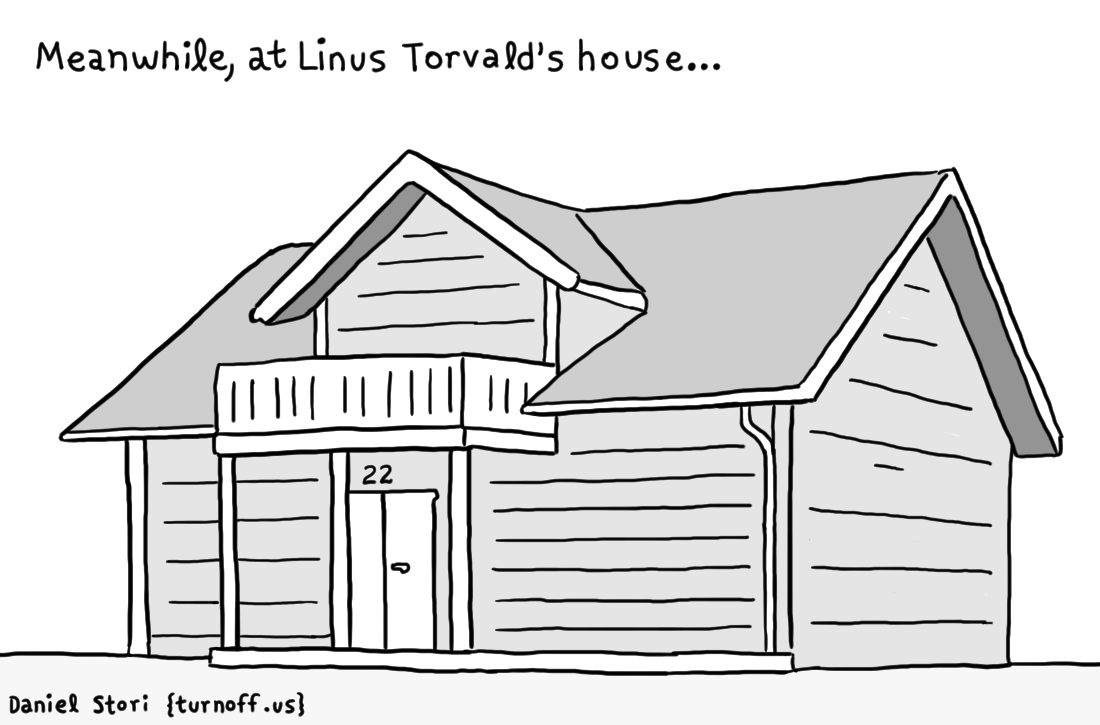
\includegraphics[scale=0.2]{linus-torvalds-house.png} \\
% ``To be a nemesis, you have to actively try to destroy something, don't you? Really, I'm not out to destroy Microsoft. That will just be a completely unintentional side effect.'' 
% \end{frame}

\begin{frame}[fragile=singleslide]{Beware Of Whitespace}
Whitespace (spaces, tabs and newlines) have more semantic content in Bash than any other language (except perhaps Haskell).
\begin{itemize}
\item Think about the way commands are structured.  A space denotes \textbf{argument application!}
\item Bash takes every character \emph{literally}! 
\end{itemize}
\begin{lstlisting}[style=terminal, language=bash]
#!/bin/bash
var2=Hello   # GOOD! 
var1 = Hello # EVIL!
\end{lstlisting}
\end{frame}

\begin{frame}[fragile=singleslide]{Bash has No Types!}
Any programmer not utterly ruined by Python knows that variables have types! 
\begin{lstlisting}[style=C, language=C]
	int var1 = 1; // This is an integer
	char[] var2 = "Hello World!"; // This is a string
	char var3 = '!'; // This is a character
\end{lstlisting}
In Bash however,
\begin{lstlisting}[style=terminal, language=bash]
var1=1 # This is some text
var2="Hello World!" # This is some text
var3='!' # This is some text
\end{lstlisting}
It is more correct to think of variables in Bash as being more like Macros in C than Variables, in that they perform \emph{direct character substitution, regardless of syntactic construction!}
\end{frame}

\begin{frame}[fragile=singleslide]{Concatenation}
Because of this, concatenation does not require an operator.  
\begin{itemize}
\item In Python, we concatenate strings like so:
\end{itemize}
\begin{lstlisting}[style=C, language=python]
var1 = "Hello, " + "World!"
\end{lstlisting}
In Bash, we just perform adjacent character substitutions:
\begin{lstlisting}[style=terminal, language=bash]
var1="Hello, "
var2="World!"
echo $var1$var2
\end{lstlisting}
Again, this is much closer to Macro programming than working with variables in a regular programming language.  
\end{frame}

\section[Substitution]{Command Substitution}
\begin{frame}[fragile=singleslide]{Command Substitution}
If you want to assign a variable to the output of a command, you need to use \textbf{command substitution}.

\begin{lstlisting}[style=terminal, language=bash]
#!/bin/bash

count=$(ls -l | grep -v total | wc -l)
echo "Number of files in directory is $count"
\end{lstlisting}
This allows you to redirect the results of \textbf{stdout} to intermediate variables, and then back into \textbf{stdin}. 
\begin{itemize}
\item You can also do this with \textbf{pipes}, which we will be covering a bit later in this course.
\end{itemize}
\end{frame}

\begin{frame}[fragile=singleslide]{Subshells}
\begin{columns}
\begin{column}{0.6\textwidth}
Code executed inside of a script is considered to be a \textbf{subshell} of the shell you execute it from.  
\end{column}
\begin{column}{0.38\textwidth}
\vspace{-0.5em}
\center
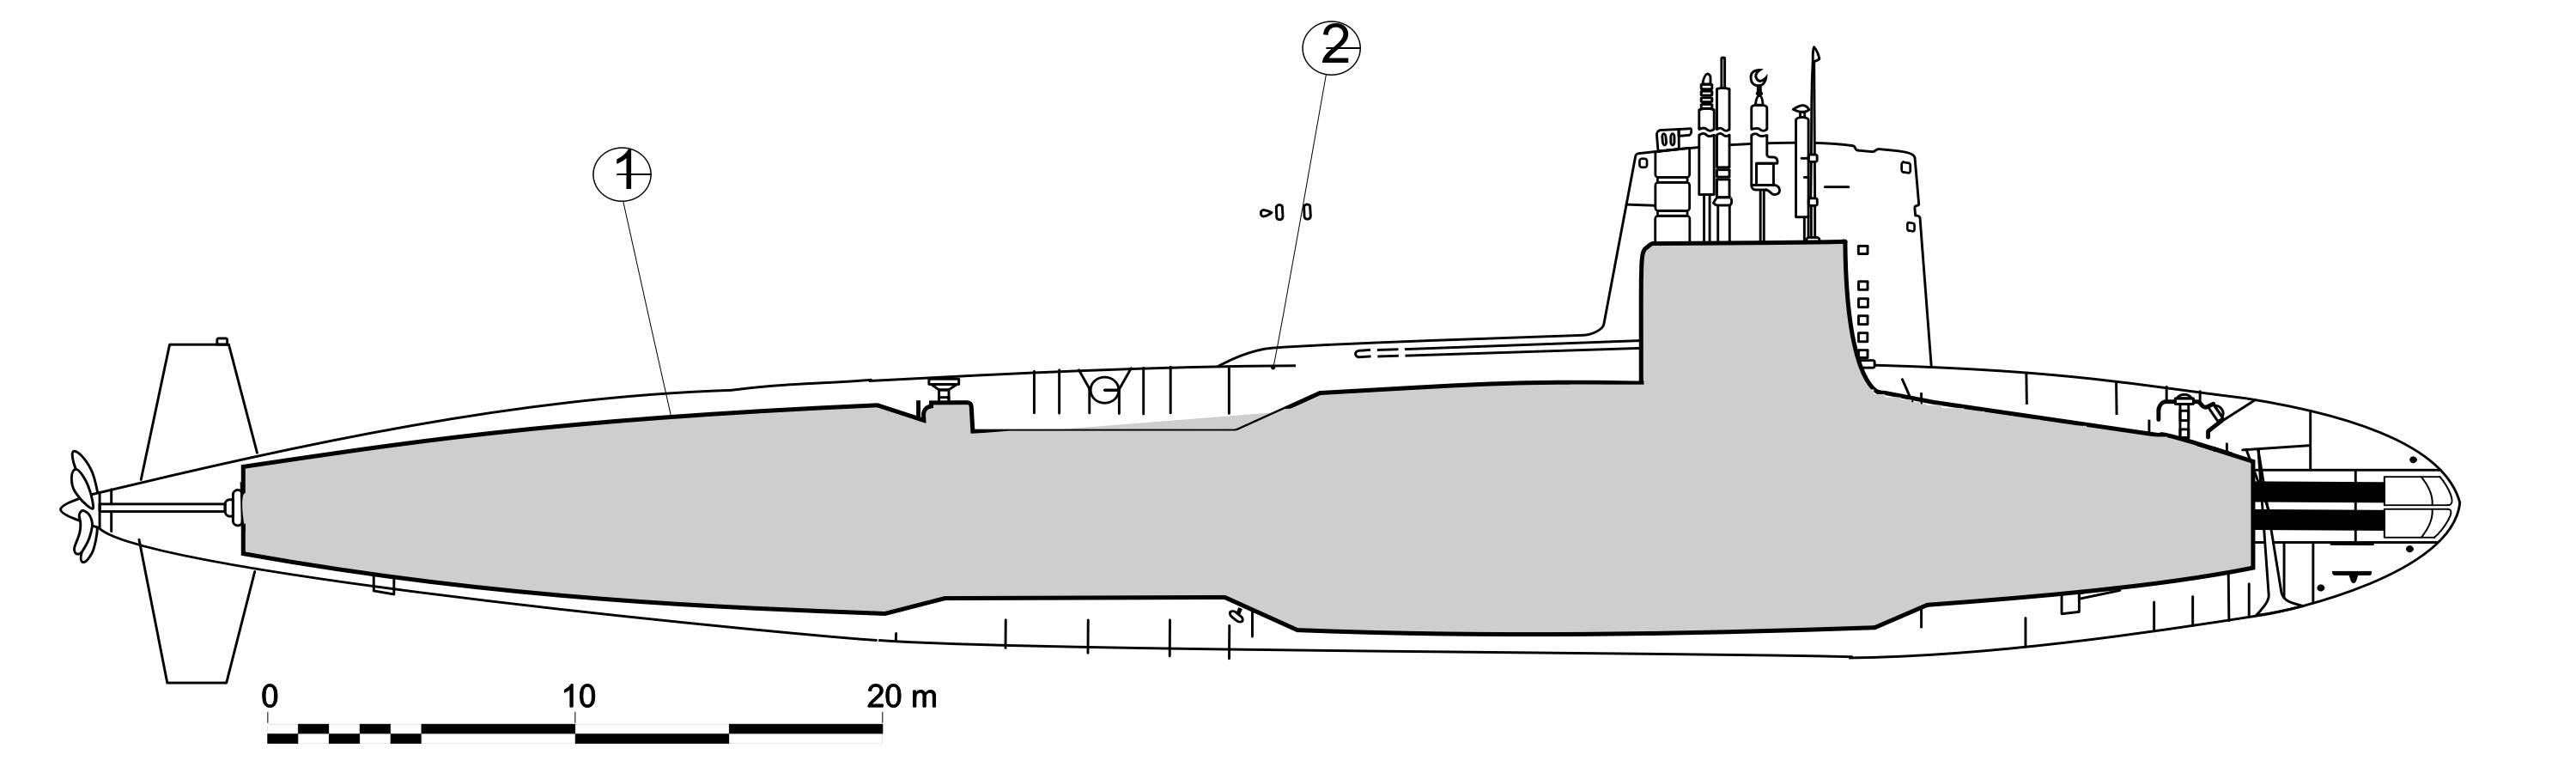
\includegraphics[scale=0.05]{subshell.png}
\end{column}
\end{columns}
\begin{itemize}
\item Variables within a shell are not automatically available within subshell processes spawned by a shell.  
\item Think of it like global variables in Python.  To use them within a function, you have to declare them!
\item Use the \texttt{export} command to accomplish this.
\end{itemize}
\begin{lstlisting}[style=terminal, language=bash]
#!/bin/bash
VAR=Hello
export VAR
./script.sh # VAR is now availabe in script.sh
\end{lstlisting}
\end{frame}

\begin{frame}[fragile=singleslide]{Expressions of Dissatisfaction}
You may be asking yourself, ``OK, but where's the MATH!?''
\begin{itemize}
\item Integer arithmetic must be performed within the \textbf{double parenthesis} envirnoment: \texttt{\$(( math goes here ))}
\item This is really just syntactic sugar for the \texttt{expr} command:
\end{itemize}
\begin{lstlisting}[style=terminal, language=bash]
RESULT1=$(( 1 + 5 ))
RESULT2=$(expr 1 + 5) # both accomplish the same thing
\end{lstlisting}
The full listing of available expressions is in the \texttt{expr} manual page!
\end{frame}

\section[Conditionals]{Conditional Control Flow}
\begin{frame}[fragile=singleslide]{If Statement Syntax}
\begin{lstlisting}[style=terminal, language=bash]
if [ <some test> ] ; then
   # some commands
fi

if [ <some test> ] && [ <another test> ] ; then
  # some commands
else 
  # some more commands
fi

if [ <some test> ] || [ <another test> ] ; then
  # some commands
elif [ <some other test> ]
  # some more commands
fi
\end{lstlisting}
\end{frame}

\begin{frame}[fragile=singleslide]{The Test Command}
\begin{lstlisting}[style=terminal, language=bash]
if [ -n "Hello" ] ; then
  echo "Hello is bigger than zero"
fi
\end{lstlisting}
\begin{itemize}
\item The square brackets \texttt{$[$ $]$} are a reference to the \texttt{test} command.
\item A full listing of the sorts of tests you can perform is in the \texttt{test} man page.  It's worth a read! 
\item The \texttt{test} command can also be used as follows.
\end{itemize}
\begin{lstlisting}[style=terminal, language=bash]
if test -n "Hello" ; then
  echo "Hello is bigger than zero"
fi
\end{lstlisting}
\end{frame}

\begin{frame}[fragile=singleslide]{Comparators!}
This is a non-exhaustive list of comparisons available in \texttt{test}.
\center
\begin{tabular}{| c | c | c |}
\hline
Operator & Data Type & Description \\ \hline \hline
\texttt{! x} & Expression & x is false \\ \hline \hline
\texttt{-n x} & String & Length of x is $\neq$ 0 \\ \hline
\texttt{x = y} & String & x and y are equal \\ \hline
\texttt{x != y} & String & x and y are not equal \\ \hline \hline
\texttt{x -eq y} & Integer & x and y are equal \\ \hline
\texttt{x -gt y} & Integer & x is greater than y \\ \hline
\texttt{x -lt y} & Integer & x is less than y \\ \hline \hline
\texttt{-e x} & Item & Item exists \\ \hline \hline
\texttt{-f x} & File & x exists and is a regular file \\ \hline
\texttt{-d x} & Directory & x exists and is a directory \\ \hline
\texttt{-x x} & File & x exists and is executable \\ \hline
\end{tabular}

\end{frame}

\section[Loops]{Iterative Control Flow}
\begin{frame}[fragile=singleslide]{Iterating the Concept}
\begin{itemize}
\item \texttt{for / in}
\begin{lstlisting}[style=terminal, language=bash]
INPUT="one two three"
for item in $INPUT ; do
  echo $item
done
\end{lstlisting}
\item C-style \texttt{for}
\begin{lstlisting}[style=terminal, language=bash]
for ((i=0 ; i < 10 ; i++)) ; do
  echo "Counter: $i"
done
\end{lstlisting}
\item \texttt{while}
\begin{lstlisting}[style=terminal, language=bash]
COUNT=0
while [ "$COUNT" -lt 10 ] ; do
  echo "$COUNT"
  COUNT=$(( $COUNT + 1 ))
done
\end{lstlisting}
\end{itemize}
\end{frame}

\begin{frame}[fragile=singleslide]{Internal Field Separation}
By default, Bash separates inputs and arguments by \emph{whitespace}.
\begin{lstlisting}[style=terminal, language=bash]
#!/bin/bash

IFS=$":"
INPUT="a:b:c:d"
for field in $INPUT; do
    echo $field
done
unset IFS

INPUT="a b c d"
for field in $INPUT; do
    echo $field
done
\end{lstlisting}

Try commenting the line \texttt{unset IFS} and see how the output changes! 
\end{frame}

% \section[Errata]{Errata}
% \begin{frame}{The Last Slide Comic}
% \center
% 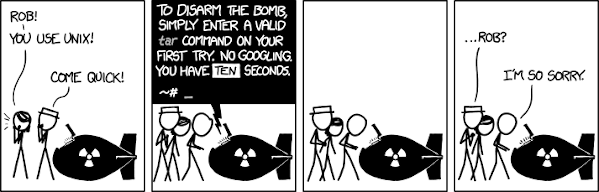
\includegraphics[scale=0.5]{tar.png}
% \end{frame}

\section[Acknowledge]{Acknowledge}
\begin{frame}{Acknowledge}
\center
\vspace{8em}
The contents of these slides were liberally borrowed (with permission) from slides from the Summer 2021 offering of 1XC3 (by Dr. Nicholas Moore).  
\end{frame}

\end{document}


